\documentclass{article}
% \usepackage{nips_2016}

% \usepackage{times}
\usepackage{amsmath}
% %\usepackage{pdfcomment}
\usepackage{amsthm,amsfonts}
\usepackage{graphicx}
% \usepackage{geometry}
% \usepackage{subcaption}
\usepackage{bm}
% \usepackage{hyperref}
% \usepackage[retainorgcmds]{IEEEtrantools}
\usepackage{xparse}
% \usepackage{mathtools}
% \usepackage{color}
% \usepackage{marginnote}
% \usepackage{booktabs}
\usepackage[utf8]{inputenc}
\usepackage{mathrsfs}
\usepackage{eufrak}
% \usepackage{enumitem}

%\usepackage{biblatex}
%\addbibresource{bibliography.bib}

\setlength{\parindent}{0em}
\setlength{\parskip}{0.8em}

\DeclareMathOperator*{\argmax}{arg\,max}
\DeclareMathOperator*{\argmin}{arg\,min}
\DeclareMathOperator*{\maximize}{maximize}
\DeclareMathOperator*{\minimize}{minimize}
\DeclareMathOperator{\st}{s.t.}
\DeclareMathOperator{\epi}{epi}
\DeclareMathOperator{\diag}{diag}
\DeclareMathOperator{\dom}{dom}
\DeclareMathOperator{\tr}{tr}
\DeclareMathOperator{\Var}{Var}
\DeclareMathOperator{\CE}{CE}
\DeclareMathOperator{\Cov}{Cov}
\DeclareMathOperator{\sign}{sign}
\DeclareMathOperator{\Pdim}{Pdim}
% \DeclareMathOperator{\E}{E}

% \DeclarePairedDelimiter\floor{\lfloor}{\rfloor}

\newcommand{\ie}{\textit{i.e.}}
\newcommand{\eg}{\textit{e.g.~}}
\newcommand{\iid}{i.i.d.~}

\newcommand{\ts}{\textsuperscript}
\newcommand{\figref}[1]{Fig.~\ref{#1}}

\newcommand{\qs}{q^\star}
\newcommand{\qsl}{q^\star_\lambda}
\newcommand{\qh}{\hat q}

\newcommand{\X}{\mathcal{X}}
\newcommand{\Y}{\mathcal{Y}}
\newcommand{\R}{\mathcal{R}}

\newcommand{\exc}{\mathscr{E}}
\renewcommand{\O}[1]{O\left(#1\right)}

\newcommand{\rad}{\hat{\mathfrak{R}}}
\newcommand{\iso}{\simeq}
\newcommand{\dd}{\partial}
\newcommand{\real}{\mathscr{R}}
\renewcommand{\Re}{\real}
\newcommand{\normal}{\mathscr{N}}
\newcommand{\trueRisk}{R_{\mathrm{true}}}
\newcommand{\uInv}{u^{-1}}
\newcommand{\qHat}{{\hat q}}
\newcommand{\qStar}{{q^\star}}
% \newcommand{\xMax}{X_{\max}}
\newcommand{\xMax}{\xi}
\newcommand{\grad}{\nabla}
% \newcommand{\dd}{\partial}
\newcommand{\E}{\bm E}
% \newcommand{\E}{E}
% \newcommand{\EU}{\bm{EU}}
\newcommand{\EU}{EU}
\newcommand{\pp}{\bm P} 
% \newcommand{\pp}{P}
% \newcommand{\CE}{\bm{CE}}
\newcommand\subsetsim{\mathrel{%
  \ooalign{\raise0.2ex\hbox{$\subset$}\cr\hidewidth\raise-0.8ex\hbox{\scalebox{0.9}{$\sim$}}\hidewidth\cr}}}

\def\rcurs{{\mbox{$\resizebox{.09in}{.08in}{\includegraphics[trim= 1em 0 14em
        0,clip]{ScriptR}}$}}}
\newcommand{\rf}{\rcurs_f}

\renewcommand{\rf}{r_0}

\newcommand{\starsection}{\vspace{1em}\begin{center}$\star\quad\star\quad\star$\end{center}\vspace{1em}}

% http://tex.stackexchange.com/questions/111551/recursive-multiple-subscript-and-superscript-with-xparse
\NewDocumentCommand{\minimizeEquationSt}{m >{\SplitList{,}}O{}}
{\text{minimize} & \quad #1\\ \text{subject to} \ProcessList{#2}{\stCommand}}
\newcommand{\minimizeEquation}[1]{\text{minimize} \quad {#1}}
\NewDocumentCommand{\stCommand}{m}
{& \quad #1}

\NewDocumentCommand{\maximizeEquationSt}{m >{\SplitList{,}}O{}}
{\text{maximize} & \quad #1\\ \text{subject to} \ProcessList{#2}{\stCommand}}
\newcommand{\maximizeEquation}[1]{\text{maximize} \quad {#1}}
% \NewDocumentCommand{\stCommand}{m}
% {& \quad #1}

\newcommand{\comment}[1]{\textbf{[#1]}}
\newcommand{\Erick}[1]{\textbf{[Erick says: #1]}}
\newcommand{\Thierry}[1]{\textbf{[Thierry says: #1]}}
\newcommand{\todo}[1]{\textbf{[Todo: #1]}}

\theoremstyle{plain}
\newtheorem{prop}{Proposition}
\newtheorem{thm}{Theorem}
\newtheorem{coro}{Corollary}
\newtheorem*{thm*}{Theorem}
\newtheorem{claim}{Claim}
\newtheorem{lemma}{Lemma}
\newtheorem*{lemma*}{Lemma}
\newtheorem{assumption}{Assumption}

\theoremstyle{definition}
\newtheorem*{definition}{Definition}
\newtheorem*{rem}{Remark}
\newtheorem*{ex}{Example}

%% http://tex.stackexchange.com/a/43971/4233
\makeatletter
\def\th@plain{%
  \thm@notefont{}% same as heading font
  \itshape % body font
}
\def\th@definition{%
  \thm@notefont{}% same as heading font
  \normalfont % body font
}
\makeatother


%%% Local Variables:
%%% mode: latex
%%% TeX-master: "article2"
%%% End:


\title{Rapport}
\author{Thierry \textsc{Bazier-Matte} \and Vincent \textsc{Johal}}
\date{Le 16 décembre 2016}

\begin{document}
\maketitle

\section{Introduction.}

\section{Calibration de la courbe zéro coupon.}

\begin{itemize}
\item Etapes de la construction de la courbe ZC.
\item Tableau des parametres
\item Tableau des erreurs de la courbe
\item Figure de la courbe ZC avec points empiriques
\item Figure de la courbe ZC NS et de la courbe forward NS
\end{itemize}

Pour construire la courbe des zéro coupons associée aux taux LIBOR et swap du marché, nous
avons.


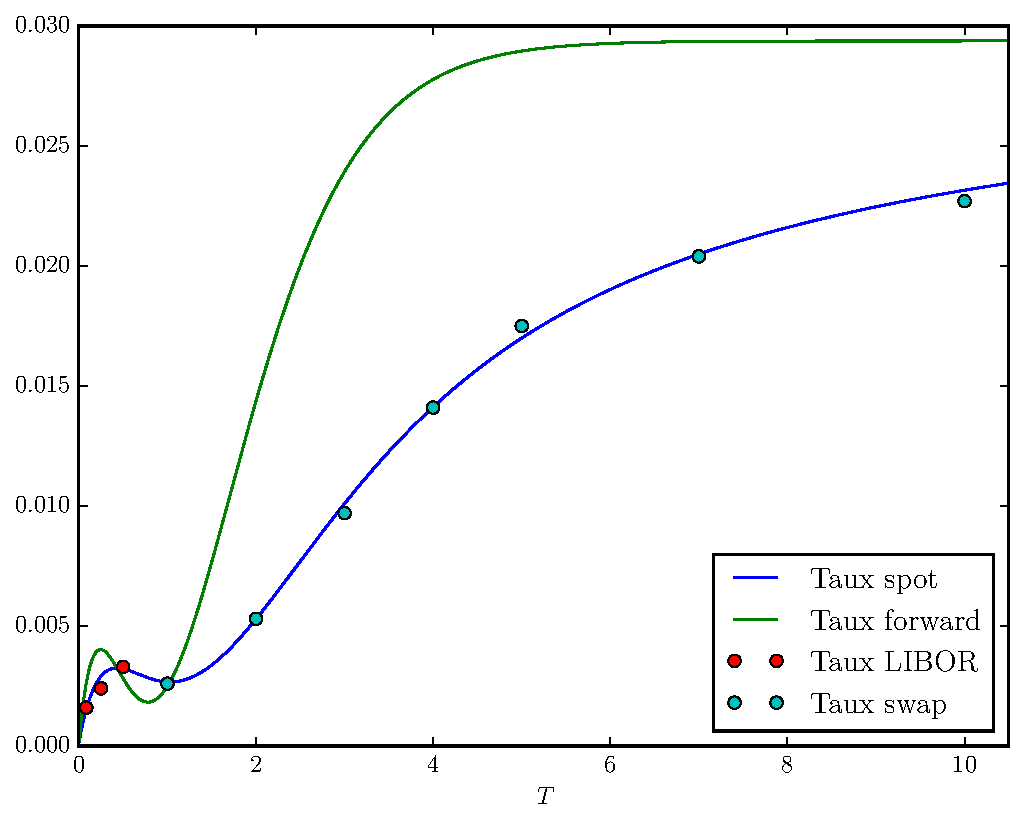
\includegraphics[width=0.3\paperwidth]{../fig/fwd_r.pdf}
%%% Local Variables:
%%% mode: latex
%%% TeX-master: "rapport"
%%% End:









\section{Calibration des prix caps.}

\begin{itemize}
\item Figure des prix caps avec le prix black.
\item Figures de la vol brutes et de la vol impliquée par le procesuss
\end{itemize}

\section{Processus CIR++.}
\begin{itemize}
\item Figures des processus dans le temps.
\item Positivité des taux et bornes employées; justification
\end{itemize}

\section{Evaluation des MBS.}


\begin{itemize}
\item Methodologie
\item Justification theorique en referant aux equation de Veronesi;
\item Insertion d'un tableau similaire a celui de la page 299;
\item Tableau des resultats et des statistiques appropriees (Deviation standard, kurtose,
  etc.)
\item Figures de la distribution et justification theorique
\item Flux financiers des IO et des PO dans le temps (voir Fig.~12.3 p. 448
  Veronesi).\cite{diebold,brigo}
\end{itemize}

% \begin{sidewaystable}
\small
\begin{tabular}{lrrrrrrr}
\toprule
{} &          $p$ &            Coupon &          Principal &   Princ. anticipé &   Int. transféré &   Princ. prépayé &             Int. \\
\midrule
0  & \num{0.0109} & \num{139861.29}\$ & \num{7326596.00}\$ & \num{103655.69}\$ & \num{33580.23}\$ & \num{79998.34}\$ & \num{36205.60}\$ \\
1  & \num{0.0105} & \num{138396.26}\$ & \num{7142941.97}\$ & \num{103098.22}\$ & \num{32738.48}\$ & \num{74821.44}\$ & \num{35298.04}\$ \\
2  & \num{0.0104} & \num{136950.19}\$ & \num{6965022.32}\$ & \num{102531.37}\$ & \num{31923.02}\$ & \num{72775.54}\$ & \num{34418.82}\$ \\
3  & \num{0.0107} & \num{135486.35}\$ & \num{6789715.40}\$ & \num{101933.84}\$ & \num{31119.53}\$ & \num{72574.37}\$ & \num{33552.51}\$ \\
4  & \num{0.0105} & \num{134067.52}\$ & \num{6615207.18}\$ & \num{101377.37}\$ & \num{30319.70}\$ & \num{69275.38}\$ & \num{32690.15}\$ \\
5  & \num{0.0107} & \num{132638.05}\$ & \num{6444554.43}\$ & \num{100791.21}\$ & \num{29537.54}\$ & \num{68713.93}\$ & \num{31846.84}\$ \\
6  & \num{0.0105} & \num{131241.82}\$ & \num{6275049.30}\$ & \num{100232.62}\$ & \num{28760.64}\$ & \num{66054.79}\$ & \num{31009.20}\$ \\
7  & \num{0.0107} & \num{129834.85}\$ & \num{6108761.88}\$ &  \num{99647.39}\$ & \num{27998.49}\$ & \num{65488.46}\$ & \num{30187.46}\$ \\
8  & \num{0.0102} & \num{128507.03}\$ & \num{5943626.03}\$ &  \num{99135.61}\$ & \num{27241.62}\$ & \num{60785.60}\$ & \num{29371.42}\$ \\
9  & \num{0.0107} & \num{127126.66}\$ & \num{5783704.82}\$ &  \num{98545.52}\$ & \num{26508.65}\$ & \num{62126.30}\$ & \num{28581.14}\$ \\
10 & \num{0.0103} & \num{125810.98}\$ & \num{5623033.00}\$ &  \num{98023.83}\$ & \num{25772.23}\$ & \num{58194.71}\$ & \num{27787.15}\$ \\
11 & \num{0.0101} & \num{124536.75}\$ & \num{5466814.47}\$ &  \num{97521.57}\$ & \num{25056.23}\$ & \num{55368.85}\$ & \num{27015.17}\$ \\
12 & \num{0.0094} & \num{123361.96}\$ & \num{5313924.05}\$ &  \num{97102.32}\$ & \num{24355.49}\$ & \num{50127.42}\$ & \num{26259.64}\$ \\
13 & \num{0.0100} & \num{122126.62}\$ & \num{5166694.31}\$ &  \num{96594.54}\$ & \num{23680.68}\$ & \num{51739.05}\$ & \num{25532.08}\$ \\
14 & \num{0.0107} & \num{120819.70}\$ & \num{5018360.72}\$ &  \num{96020.63}\$ & \num{23000.82}\$ & \num{53703.34}\$ & \num{24799.07}\$ \\
15 & \num{0.0103} & \num{119571.10}\$ & \num{4868636.74}\$ &  \num{95511.92}\$ & \num{22314.59}\$ & \num{50314.29}\$ & \num{24059.18}\$ \\
16 & \num{0.0097} & \num{118415.24}\$ & \num{4722810.53}\$ &  \num{95076.68}\$ & \num{21646.21}\$ & \num{45654.27}\$ & \num{23338.56}\$ \\
17 & \num{0.0096} & \num{117281.87}\$ & \num{4582079.57}\$ &  \num{94638.76}\$ & \num{21001.20}\$ & \num{43855.83}\$ & \num{22643.11}\$ \\
18 & \num{0.0097} & \num{116147.35}\$ & \num{4443584.98}\$ &  \num{94188.64}\$ & \num{20366.43}\$ & \num{42984.56}\$ & \num{21958.72}\$ \\
19 & \num{0.0101} & \num{114971.57}\$ & \num{4306411.78}\$ &  \num{93690.72}\$ & \num{19737.72}\$ & \num{43594.54}\$ & \num{21280.85}\$ \\
20 & \num{0.0105} & \num{113762.64}\$ & \num{4169126.52}\$ &  \num{93160.21}\$ & \num{19108.50}\$ & \num{43838.56}\$ & \num{20602.43}\$ \\
21 & \num{0.0101} & \num{112611.97}\$ & \num{4032127.76}\$ &  \num{92686.54}\$ & \num{18480.59}\$ & \num{40783.50}\$ & \num{19925.43}\$ \\
22 & \num{0.0095} & \num{111543.35}\$ & \num{3898657.71}\$ &  \num{92277.48}\$ & \num{17868.85}\$ & \num{36996.09}\$ & \num{19265.87}\$ \\
23 & \num{0.0091} & \num{110530.44}\$ & \num{3769384.14}\$ &  \num{91903.40}\$ & \num{17276.34}\$ & \num{34229.15}\$ & \num{18627.04}\$ \\
24 & \num{0.0090} & \num{109538.32}\$ & \num{3643251.58}\$ &  \num{91534.58}\$ & \num{16698.24}\$ & \num{32701.98}\$ & \num{18003.73}\$ \\
25 & \num{0.0089} & \num{108561.34}\$ & \num{3519015.02}\$ &  \num{91171.54}\$ & \num{16128.82}\$ & \num{31386.20}\$ & \num{17389.80}\$ \\
26 & \num{0.0085} & \num{107641.81}\$ & \num{3396457.28}\$ &  \num{90857.65}\$ & \num{15567.10}\$ & \num{28768.46}\$ & \num{16784.16}\$ \\
27 & \num{0.0080} & \num{106784.64}\$ & \num{3276831.17}\$ &  \num{90591.64}\$ & \num{15018.81}\$ & \num{26093.93}\$ & \num{16193.01}\$ \\
28 & \num{0.0068} & \num{106055.94}\$ & \num{3160145.60}\$ &  \num{90439.55}\$ & \num{14484.00}\$ & \num{21564.96}\$ & \num{15616.39}\$ \\
29 & \num{0.0074} & \num{105273.81}\$ & \num{3048141.08}\$ &  \num{90210.91}\$ & \num{13970.65}\$ & \num{22479.17}\$ & \num{15062.90}\$ \\
30 & \num{0.0072} & \num{104518.86}\$ & \num{2935451.00}\$ &  \num{90012.84}\$ & \num{13454.15}\$ & \num{21050.91}\$ & \num{14506.02}\$ \\
31 & \num{0.0069} & \num{103802.24}\$ & \num{2824387.25}\$ &  \num{89845.06}\$ & \num{12945.11}\$ & \num{19365.05}\$ & \num{13957.18}\$ \\
32 & \num{0.0066} & \num{103117.17}\$ & \num{2715177.15}\$ &  \num{89699.67}\$ & \num{12444.56}\$ & \num{17919.53}\$ & \num{13417.50}\$ \\
33 & \num{0.0060} & \num{102495.45}\$ & \num{2607557.95}\$ &  \num{89609.76}\$ & \num{11951.31}\$ & \num{15721.77}\$ & \num{12885.68}\$ \\
34 & \num{0.0060} & \num{101877.47}\$ & \num{2502226.41}\$ &  \num{89512.30}\$ & \num{11468.54}\$ & \num{15086.69}\$ & \num{12365.17}\$ \\
35 & \num{0.0060} & \num{101263.22}\$ & \num{2397627.42}\$ &  \num{89414.94}\$ & \num{10989.13}\$ & \num{14456.03}\$ & \num{11848.28}\$ \\
\bottomrule
\end{tabular}

\normalsize
% \end{sidewaystable}

%%% Local Variables:
%%% mode: latex
%%% TeX-master: "rapport"
%%% End:


\section{Evaluation de la durée.}
\begin{itemize}
\item Justification theorique (pourquoi le $\delta$).
\item Tableau des resultats et methodologie
\end{itemize}

\section{Conclusion.}

Ceci est un test.

Une couleur foncée.


\bibliographystyle{abbrv}
\bibliography{biblio}


\end{document}




